%% Encoding: ISO8859-1 %%

\section{Motivation}
\subsection{General}
\frame{
\frametitle{Motivation}
\begin{itemize}
\item ASR and SLT commercially great success [''OK, Google``, Siri, Jibbigo]
\pause
\item Best performing ASR models are still trained on one source language.\cite{tang2016multi}
\end{itemize}
\hrulefill
\pause
\begin{itemize}
\item Performance increase for multilingual tasks\cite{tang2016multi}, UI streamlining.
\end{itemize}
}
\subsection{Applications}
\frame{
\frametitle{Specific Applications}
\begin{block}{
\includegraphics[width=0.85\textwidth,height=0.075\textwidth]{bilder/lectureTranslator}}
\begin{center}
\begin{itemize}
\item Low latency, online application
\pause
\item Small source language amount make performance increase likely
\end{itemize}
\end{center}
\end{block}
\pause
\begin{block}{
\includegraphics[width=0.2\textwidth,height=0.08\textwidth]{bilder/EUParl}\huge{European Parliament}}
\begin{center}
\begin{itemize}
\item Attempts to replace translators with SLT \cite{tcstar}
\pause
\item Many languages challenging, great potential.
\end{itemize}
\end{center}
\end{block}
}

\section{Related Work}
\frame{
\frametitle{Related Work}
\begin{block}{Non-NN-Approaches}
\begin{center}
\begin{itemize}
\item single-language phone recognition followed by language-dependent,
interpolated n-gram language modeling (PRLM)\cite{zissman1996comparison}
\item multiple single-language phone recognizers and language-dependent parallel phone recognition (PPRM)\cite{zissman1996comparison}
\item Gaussian Mixture Models (GMM)s \cite{torres2002approaches}
\item Vector Space Modelling + PPRM\cite{4032773}
\item I-Vector approaches\cite{6680440}\cite{d2012phonotactic}
\end{itemize}
\end{center}
\end{block}
}
\frame{
\frametitle{Related Work II/Based on}
\begin{block}{Similar Approaches}
\begin{center}
\begin{itemize}
\item Matejka et. al\cite{matejka2014neural} similar setup: BNF \(\rightarrow\) LID, with averaging 5 LID nets. 
\item \cite{6289007} M. Heck et al. evaluate LID approaches prospect of Lecture Translator integration: PPRM/PRLM + Hybrid.
\end{itemize}
\end{center}
\end{block}
\hrulefill
\pause
\begin{itemize}
\item Markus \cite{Mueller2016b}: ''Language Adaptive DNNs for Improved Low Resource Speech Recognition``, experimental setup very similar (LFV/LID)
\end{itemize}
}

\section{Experimental Setup}
\subsection{Overview}
\frame{
\frametitle{Experimental Setup}
\tikzstyle{layer}=[draw=black,fill=black!30]
\tikzstyle{layerlid}=[draw=black,fill=green!30]
\tikzstyle{dots}=[draw=black,fill=black]

   \begin{tikzpicture}[scale=0.8]

   % Acoustic feature stack

   \draw (-1.75, 2.5) node[draw=white,fill=white] {AF stack};
   \fill[layer] (-2,1) coordinate(l0bl) -- (-1.5,1) coordinate(l0br) --
(-1.5,2) coordinate(l0tr) -- (-2,2) coordinate(l0tl) -- (-2,1);

   \fill[layer] (-2,0) coordinate(l0_1bl) -- (-1.5,0) coordinate(l0_1br)
-- (-1.5,1) coordinate(l0_1tr) -- (-2,1) coordinate(l0_1tl) -- (-2,0);

   \draw[dots] (-1.75,-0.2) circle (0.045);
   \draw[dots] (-1.75,-0.375) circle (0.045);
   \draw[dots] (-1.75,-0.55) circle (0.045);

   \fill[layer] (-2,-1.75) coordinate(l0_2bl) -- (-1.5,-1.75)
coordinate(l0_2br) -- (-1.5,-0.75) coordinate(l0_2tr) -- (-2,-0.75)
coordinate(l0_2tl) -- (-2,-1.75);

   % Bottle-neck stack

   \fill[layer] (4,-1.5) coordinate(l5_1bl) -- (4.5,-1.5)
coordinate(l5_1br) -- (4.5,-0.5) coordinate(l5_1tr) -- (4,-0.5)
coordinate(l5_1tl) -- (4,-1.5);

   \draw[dots] (4.25,-1.7) circle (0.045);
   \draw[dots] (4.25,-1.875) circle (0.045);
   \draw[dots] (4.25,-2.05) circle (0.045);

   \fill[layer] (4,-3.25) coordinate(l5_2bl) -- (4.5,-3.25)
coordinate(l5_2br) -- (4.5,-2.25) coordinate(l5_2tr) -- (4,-2.25)
coordinate(l5_2tl) -- (4,-3.25);

   \draw (1.5,-2.25) node {DBNF};

   \draw (4.25,2.5) node[draw=white,fill=white] {BNF stack};

   % BNF Layers

   \fill[layer] (4,-0.5) coordinate(l5bl) -- (4.5,-0.5) coordinate(l5br)
-- (4.5,0.5) coordinate(l5tr) -- (4,0.5) coordinate(l5tl) -- (4,-0.5);
   \fill[layer] (2.5,-1.5) coordinate(l4bl) -- (3,-1.5) coordinate(l4br)
-- (3,1.5) coordinate(l4tr) -- (2.5,1.5) coordinate(l4tl) -- (2.5,-1.5);

   \draw[dots] (2,0) circle (0.045);
   \draw[dots] (2.175,0) circle (0.045);
   \draw[dots] (1.825,0) circle (0.045);

   \fill[layer] (1,-1.5) coordinate(l2bl) -- (1.5,-1.5) coordinate(l2br)
-- (1.5,1.5) coordinate(l2tr) -- (1,1.5) coordinate(l2tl) -- (1,-1.5);
   \fill[layer] (0,-1.5) coordinate(l1bl) -- (0.5,-1.5) coordinate(l1br)
-- (0.5,1.5) coordinate(l1tr) -- (0,1.5) coordinate(l1tl) -- (0,-1.5);

   \draw (l0tr) -- (l1bl);
   \draw (l0_2br) -- (l1tl);
   \draw (l1tr) -- (l2bl);
   \draw (l1br) -- (l2tl);
   \draw (l4tr) -- (l5bl);
   \draw (l4br) -- (l5tl);


   % DNN Layers

   \fill[layer] (6,-3) coordinate(l6bl) -- (6.5,-3) coordinate(l6br) --
(6.5,0) coordinate(l6tr) -- (6,0) coordinate(l6tl) -- (6,-3);
   \fill[layer] (7,-3) coordinate(l7bl) -- (7.5,-3) coordinate(l7br) --
(7.5,0) coordinate(l7tr) -- (7,0) coordinate(l7tl) -- (7,-3);

   \draw[dots] (8,-1.5) circle (0.045);
   \draw[dots] (8.175,-1.5) circle (0.045);
   \draw[dots] (7.825,-1.5) circle (0.045);

   \fill[layer] (8.5,-3) coordinate(l11bl) -- (9,-3) coordinate(l11br)
-- (9,0) coordinate(l11tr) -- (8.5,0) coordinate(l11tl) -- (8.5,-3);
   \fill[layer] (10.5,-2) coordinate(l12bl) -- (11,-2) coordinate(l12br)
-- (11,-1) coordinate(l12tr) -- (10.5,-1) coordinate(l12tl) -- (10.5,-1);

   \draw (10.75,2.5) node[draw=white,fill=white] {LID};

   \draw (l5tr) -- (l6bl);
   \draw (l5_2br) -- (l6tl);

   \draw (l6tr) -- (l7bl);
   \draw (l6br) -- (l7tl);
   \draw (l11tr) -- (l12bl);
   \draw (l11br) -- (l12tl);

   \draw (l12tl) -- (l12bl);

   \draw (7.5,-3.75) node {Language Identity Network};

   \end{tikzpicture}
}
\subsection{Data Sets}
\frame{
\frametitle{Data Sets}
\begin{block}{Euronews 2014}
\begin{center}
\begin{itemize}
\item 10 Languages (EN, FR, DE, AR, ES, IT, PO, PT, RU, TR)
\item Original Corpus: 72h / Language, Reduced corpus: 18h / Language (Random Sampling of 10.000 speakers)
\item 80 \% train data, 10 \% each dev/test set
\end{itemize}
\end{center}
\end{block}
\pause
\begin{block}{Lecture Data}
\begin{center}
\begin{itemize}
\item 3 Languages (EN, FR, DE) \(\approx\)10h per language.
\item KIT lectures, InterACT25, DGA talks
\item Validation of Euronews results, ``right'' patterns learned (different environment)
\end{itemize}
\end{center}
\end{block}
}
\frame{
\frametitle{Data Sets II}
\begin{block}{European Parliament}
\begin{center}
\begin{itemize}
\item 7 Languages (EN, FR, DE, ES, IT, PO, PT) 3.6h per language
\item Simultaneous translation of all parliament speeches
\item Further Validation, Proof-of-concept for Lecture Translator integration
\end{itemize}
\end{center}
\end{block}
}
\subsection{Feature Extraction}
\frame{
\frametitle{Feature Extraction}
\begin{block}{Feature Definition}
\begin{center}
\begin{itemize}
\item Samplerate: 16 kHz
\pause
\item Standard Janus Capabilities: 
\begin{itemize}
\item POWER
\item lMEL
\item PITCH
\item TONE
\end{itemize}
\pause
\item Context of 6 frames
\end{itemize}
\end{center}
\end{block}
}
\frame{
\frametitle{DBNF}
\begin{columns}[t,onlytextwidth]
\column{.5\textwidth}
\tikzstyle{layer}=[draw=black,fill=black!30]
\tikzstyle{layerlid}=[draw=black,fill=green!30]
\tikzstyle{dots}=[draw=black,fill=black]
\begin{tikzpicture}[scale=0.8,baseline=(current bounding box.north)]

   % Bottle-neck stack


   \draw (1.5,-2.25) node {DBNF};
% BNF Layers

   \fill[layer] (2.5,-1.5) coordinate(l4bl) -- (3,-1.5) coordinate(l4br)
-- (3,1.5) coordinate(l4tr) -- (2.5,1.5) coordinate(l4tl) -- (2.5,-1.5);

   \draw[dots] (2,0) circle (0.045);
   \draw[dots] (2.175,0) circle (0.045);
   \draw[dots] (1.825,0) circle (0.045);

   \fill[layer] (1,-1.5) coordinate(l2bl) -- (1.5,-1.5) coordinate(l2br)
-- (1.5,1.5) coordinate(l2tr) -- (1,1.5) coordinate(l2tl) -- (1,-1.5);
   \fill[layer] (0,-1.5) coordinate(l1bl) -- (0.5,-1.5) coordinate(l1br)
-- (0.5,1.5) coordinate(l1tr) -- (0,1.5) coordinate(l1tl) -- (0,-1.5);

   \draw (l1tr) -- (l2bl);
   \draw (l1br) -- (l2tl);

\end{tikzpicture}
\column{.5\textwidth}
\begin{center}
\begin{block}{DBNF}
\begin{center}
\begin{itemize}
\item AF Stack as input
\pause
\item Targets context-dependent phoneme states
\pause
\item 6 layers, each 1000 neurons
\pause
\item BNF of 42 dimensions
\pause
\item Stacked with context of 11 frames
\end{itemize}
\end{center}
\end{block}
\end{center}
\end{columns}
}
\subsection{DNN structure}
\frame{
\frametitle{Context Spread}
\begin{columns}[t,onlytextwidth]
\column{.5\textwidth}
\tikzstyle{frame}=[draw=black,fill=black!80]
\tikzstyle{framespread}=[draw=black,fill=black!10]
\tikzstyle{dots}=[draw=black,fill=black]
\begin{tikzpicture}[scale=0.8,baseline=(current bounding box.north)]

%%%% SPREAD 1
\draw (1.5,-1.0) node {Spread of 1};

 \draw[dots] (-1.05,0) circle (0.045);
 \draw[dots] (-0.7,0) circle (0.045);
 \draw[dots] (-0.35,0) circle (0.045);

\fill[frame] (0,-0.5) coordinate(l1bl) -- (0.5,-0.5) coordinate(l1br)
-- (0.5,0.5) coordinate(l1tr) -- (0,0.5) coordinate(l1tl) -- (0,0.5);

\fill[frame] (0.75,-0.5) coordinate(l2bl) -- (1.25,-0.5) coordinate(l2br)
-- (1.25,0.5) coordinate(l2tr) -- (0.75,0.5) coordinate(l2tl) -- (0.75,0.5);

\fill[frame] (1.5,-0.5) coordinate(l3bl) -- (2,-0.5) coordinate(l3br)
-- (2.0,0.5) coordinate(l3tr) -- (1.5,0.5) coordinate(l3tl) -- (1.5,0.5);

\fill[frame] (2.25,-0.5) coordinate(l4bl) -- (2.75,-0.5) coordinate(l4br)
-- (2.75,0.5) coordinate(l4tr) -- (2.25,0.5) coordinate(l4tl) -- (2.25,0.5);

\fill[frame] (3,-0.5) coordinate(l5bl) -- (3.5,-0.5) coordinate(l5br)
-- (3.5,0.5) coordinate(l5tr) -- (3,0.5) coordinate(l5tl) -- (3,0.5);

 \draw[dots] (3.85,0) circle (0.045);
 \draw[dots] (4.2,0) circle (0.045);
 \draw[dots] (4.55,0) circle (0.045);

%%%% SPREAD 2
\draw (1.5,-3) node {Spread of 2};

 \draw[dots] (-1.05,-2) circle (0.045);
 \draw[dots] (-0.7,-2) circle (0.045);
 \draw[dots] (-0.35,-2) circle (0.045);

\fill[frame] (0,-2.5) coordinate(l6bl) -- (0.5,-2.5) coordinate(l6br)
-- (0.5,-1.5) coordinate(l6tr) -- (0,-1.5) coordinate(l6tl) -- (0,-1.5);

\fill[framespread] (0.75,-2.5) coordinate(l7bl) -- (1.25,-2.5) coordinate(l7br)
-- (1.25,-1.5) coordinate(l7tr) -- (0.75,-1.5) coordinate(l7tl) -- (0.75,-1.5);

\fill[frame] (1.5,-2.5) coordinate(l8bl) -- (2,-2.5) coordinate(l8br)
-- (2.0,-1.5) coordinate(l8tr) -- (1.5,-1.5) coordinate(l8tl) -- (1.5,-1.5);

\fill[framespread] (2.25,-2.5) coordinate(l9bl) -- (2.75,-2.5) coordinate(l9br)
-- (2.75,-1.5) coordinate(l9tr) -- (2.25,-1.5) coordinate(l9tl) -- (2.25,-1.5);

\fill[frame] (3,-2.5) coordinate(l10bl) -- (3.5,-2.5) coordinate(l10br)
-- (3.5,-1.5) coordinate(l10tr) -- (3,-1.5) coordinate(l10tl) -- (3,-1.5);

 \draw[dots] (3.85,-2) circle (0.045);
 \draw[dots] (4.2,-2) circle (0.045);
 \draw[dots] (4.55,-2) circle (0.045);

%%%% SPREAD 3
\draw (1.5,-5) node {Spread of 3};

 \draw[dots] (-1.05,-4) circle (0.045);
 \draw[dots] (-0.7,-4) circle (0.045);s
 \draw[dots] (-0.35,-4) circle (0.045);

\fill[frame] (0,-4.5) coordinate(l11bl) -- (0.5,-4.5) coordinate(l11br)
-- (0.5,-3.5) coordinate(l11tr) -- (0,-3.5) coordinate(l11tl) -- (0,-3.5);

\fill[framespread] (0.75,-4.5) coordinate(l12bl) -- (1.25,-4.5) coordinate(l12br)
-- (1.25,-3.5) coordinate(l12tr) -- (0.75,-3.5) coordinate(l12tl) -- (0.75,-3.5);

\fill[framespread] (1.5,-4.5) coordinate(l13bl) -- (2,-4.5) coordinate(l13br)
-- (2.0,-3.5) coordinate(l13tr) -- (1.5,-3.5) coordinate(l13tl) -- (1.5,-3.5);

\fill[frame] (2.25,-4.5) coordinate(l14bl) -- (2.75,-4.5) coordinate(l14br)
-- (2.75,-3.5) coordinate(l14tr) -- (2.25,-3.5) coordinate(l14tl) -- (2.25,-3.5);

\fill[framespread] (3,-4.5) coordinate(l15bl) -- (3.5,-4.5) coordinate(l15br)
-- (3.5,-3.5) coordinate(l15tr) -- (3,-3.5) coordinate(l15tl) -- (3,-3.5);

 \draw[dots] (3.85,-4) circle (0.045);
 \draw[dots] (4.2,-4) circle (0.045);
 \draw[dots] (4.55,-4) circle (0.045);


%% fix missing links
   \draw (l1tl) -- (l1bl);
   \draw (l2tl) -- (l2bl);
   \draw (l3tl) -- (l3bl);
   \draw (l4tl) -- (l4bl);
   \draw (l5tl) -- (l5bl);
   \draw (l6tl) -- (l6bl);
   \draw (l7tl) -- (l7bl);
   \draw (l8tl) -- (l8bl);
   \draw (l9tl) -- (l9bl);
   \draw (l10tl) -- (l10bl);
   \draw (l11tl) -- (l11bl);
   \draw (l12tl) -- (l12bl);
   \draw (l13tl) -- (l13bl);
   \draw (l14tl) -- (l14bl);
   \draw (l15tl) -- (l15bl);

\end{tikzpicture}
\column{.5\textwidth}
\begin{block}{Spread Evaluation}
\begin{center}
\begin{itemize}
\item In \cite{Mueller2016b}, evaluated spreads of 2,3,6 for LFV
\pause
\item Evaluation of spreads 4 and 5 for different nets on Euronews
\pause
\item Spread of 3 outperforms 4 and 5, surprisingly 5 outperforms 4
\end{itemize}
\end{center}
\end{block}
\end{columns}
}
\frame{
\frametitle{DNN Structure}
\begin{columns}[t,onlytextwidth]
\column{.5\textwidth}
\tikzstyle{layer}=[draw=black,fill=black!30]
\tikzstyle{layerlid}=[draw=black,fill=green!30]
\tikzstyle{dots}=[draw=black,fill=black]
\begin{tikzpicture}[scale=0.8,baseline=(current bounding box.north)]
% DNN Layers

   \fill[layer] (6,-3) coordinate(l6bl) -- (6.5,-3) coordinate(l6br) --
(6.5,0) coordinate(l6tr) -- (6,0) coordinate(l6tl) -- (6,-3);
   \fill[layer] (7,-3) coordinate(l7bl) -- (7.5,-3) coordinate(l7br) --
(7.5,0) coordinate(l7tr) -- (7,0) coordinate(l7tl) -- (7,-3);

   \draw[dots] (8,-1.5) circle (0.045);
   \draw[dots] (8.175,-1.5) circle (0.045);
   \draw[dots] (7.825,-1.5) circle (0.045);

   \fill[layer] (8.5,-3) coordinate(l11bl) -- (9,-3) coordinate(l11br)
-- (9,0) coordinate(l11tr) -- (8.5,0) coordinate(l11tl) -- (8.5,-3);
   \fill[layer] (10.5,-2) coordinate(l12bl) -- (11,-2) coordinate(l12br)
-- (11,-1) coordinate(l12tr) -- (10.5,-1) coordinate(l12tl) -- (10.5,-1);

   \draw (10.75,2.5) node[draw=white,fill=white] {LID};
\draw (l11tr) -- (l12bl);
   \draw (l11br) -- (l12tl);
\draw (l12tl) -- (l12bl);

\end{tikzpicture}
\column{.5\textwidth}
\begin{center}
\begin{block}{Baseline Setup}
\begin{center}
\begin{itemize}
\item BNF with context as input
\pause
\item 5 layers of each 1000 neurons
\pause
\item Tanh activation, mse loss function
\pause
\item Mini-batches size 2,000,000, learning rate(lr) 0.01
\pause
\item Retrained with 1000:10 layer with lr 1
\end{itemize}
\end{center}
\end{block}
\end{center}
\end{columns}
}
\section{DNN Structure}
\frame{
\frametitle{Evaluating Different Net Structures}
\begin{columns}[t,onlytextwidth]
\column{.5\textwidth}
\tikzstyle{layer}=[draw=black,fill=black!30]
\tikzstyle{layerlid}=[draw=black,fill=green!30]
\tikzstyle{dots}=[draw=black,fill=black]
   \begin{tikzpicture}[scale=0.8,baseline=(current bounding box.north)]


   \fill[layer] (0,-1.5) coordinate(l1bl) -- (0.5,-1.5) coordinate(l1br)
-- (0.5,1.5) coordinate(l1tr) -- (0,1.5) coordinate(l1tl) -- (0,-1.5);
   \fill[layer] (1,-1.25) coordinate(l2bl) -- (1.5,-1.25) coordinate(l2br)
-- (1.5,1.25) coordinate(l2tr) -- (1,1.25) coordinate(l2tl) -- (1,-1.25);
   \fill[layer] (2,-1.0) coordinate(l3bl) -- (2.5,-1.0) coordinate(l3br)
-- (2.5,1.0) coordinate(l3tr) -- (2,1.0) coordinate(l3tl) -- (2,-1.0);

   \draw[dots] (2.625,0) circle (0.045);
   \draw[dots] (2.75,0) circle (0.045);
   \draw[dots] (2.875,0) circle (0.045);




   \fill[layer] (3,-0.25) coordinate(l4bl) -- (3.5,-0.25) coordinate(l4br)
-- (3.5,0.25) coordinate(l4tr) -- (3,0.25) coordinate(l4tl) -- (3,-0.25);
\end{tikzpicture}
\column{.5\textwidth}
\begin{center}
\begin{block}{Other Evaluations}
\begin{center}
\begin{itemize}
\item Lower LR \checkmark
\pause
\item Baseline add Layers \xmark
\pause
\item \color{black}{Tree net with 5 layers} \checkmark
\pause
\item \color{black}{Tree net with 6 layers} \checkmark
\pause
\item \color{black}{Tree net with \(>\) 6 layers} \xmark
\pause
\item \color{black}{Cross-Data-Set training} \checkmark
\pause
\item \color{black}{Concat-Set training} \checkmark \checkmark
\end{itemize}
\end{center}
\end{block}
\end{center}
\end{columns}
}
\section{Post Processing}
\subsection{Motivation}
\frame{
\frametitle{Output}
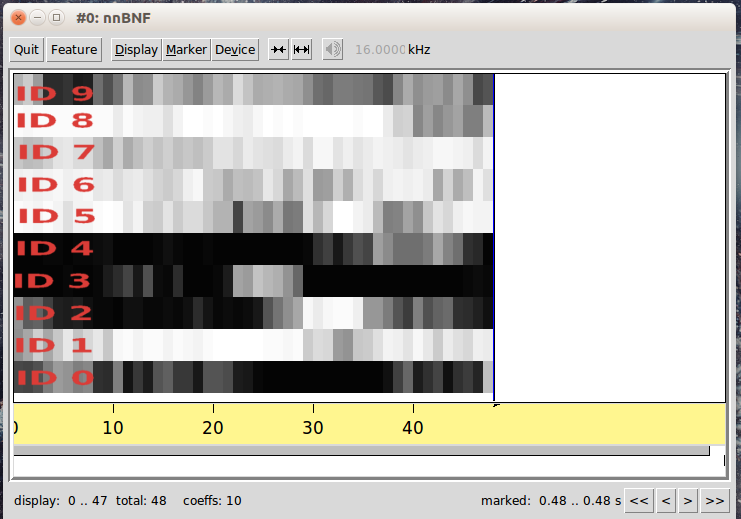
\includegraphics[width=0.7\textwidth]{bilder/frenchCorrect}

}

\frame{
\frametitle{Output}
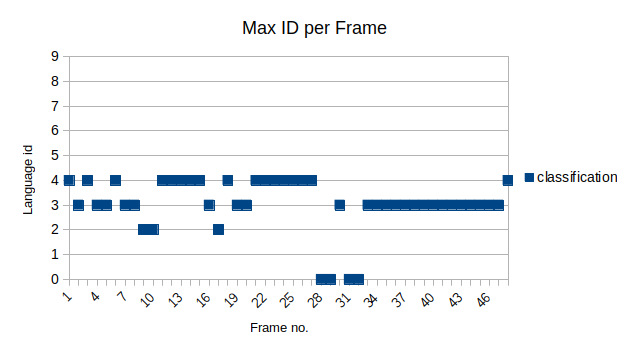
\includegraphics[width=1.0\textwidth]{bilder/cleaned}

}

\subsection{Smoothing Filters}
\frame{
\frametitle{Metrics}
\begin{exampleblock}{Error Rate}
\begin{center}
\begin{itemize}
\item Count outputs per language per frame
\item Max count == actual language \(\rightarrow\) correct, false otherwise
\item Metric is percentage of error per language
\end{itemize}
\end{center}
\end{exampleblock}
\pause
\begin{exampleblock}{Out-Of-Language-Error (OLE)}
\begin{center}
\begin{itemize}
\item Same counting as before
\item Sum up FALSELY (as not equal to max language) classified languages
\item Metric of ``Sureness'' of output
\item Example: 50 frames classified as DE, 10 as EN, 5 as FR: \((5+10)/(5+10+50) = 0.23\)
\item Average OLE per language
\end{itemize}
\end{center}
\end{exampleblock}
}

\frame{
\frametitle{Smoothing Filters}
\begin{block}{Approaches}
\begin{center}
\begin{itemize}
\item Counting Filter (count in window, in total as maximum only).
\item Gaussian Filter (convolution with Gaussian kernel)
\item Speech / Noise Filter
\item Language Filter (If domain smaller than targets trained)
\item Sequence Filter (longest sequence in window)
\item Difference (Only count output if difference between 2 max is \(>\) thresh
\item Weighted Average (FILTER capability)
\end{itemize}
\end{center}
\end{block}
}
\section{Results}
\frame{
\frametitle{Results I}
\begin{tabular}{| l | c | r |}
	\hline
	\textbf{Filter} & \textbf{Overall Error TEST} & \textbf{OLE TEST} \\
	\hline
	Bare Net & 0.305 & 0.198 \\
	\hline
	Gaussian Filter (WS 15) & \textbf{0.307}  & 0.176 \\
	\hline
	Counting Filter (WS 100) & \textbf{0.307} & \textbf{0.006} \\
	\hline
	\textbf{Best} & \textbf{0.307} & \textbf{0.006} \\
	\hline
\end{tabular}
}

\frame{
\frametitle{Results II}
\begin{center}
\begin{itemize}
\item Euronews: Samples \(>\) 500 ms: 16 \% Error (10L)
\item Lecture Data: 6.5 \% Error (3L, concat with Euronews data)
\item European Parliament: 35 \% (7L, 3.5h/language)
\item Post Processing: Counting, Gauss Filter promising, relative improvement OLE 97 \%.
\end{itemize}
\end{center}
}

\subsection{Demo}
\frame{
\frametitle{Demo (easy)}
\visible<1-1>{\movie[inlinesound, samplingrate=16000,bitspersample=16]{\fbox{Play}}{15.mp3}}
\visible<2->{\begin{tabular}{| l |  r |}
\hline
\textbf{Language} & \textbf{Number of Frames classified} \\
\hline
English & 1095 \\
German & 123 \\
French & 18 \\
\hline
\textbf{Total Error} & 0.11 \\
\hline
\end{tabular}}
}

\frame{
\frametitle{Demo (difficult)}
\visible<1-1>{\movie[inlinesound, samplingrate=16000,bitspersample=16]{\fbox{Play}}{iwslt14Le.mp3}}
\visible<2->{\begin{tabular}{| l |  r |}
\hline
\textbf{Language} & \textbf{Number of Frames classified} \\
\hline
English & 435 \\
German & 53 \\
French & 99\\
\hline
\textbf{Total Error} & 0.25 \\
\hline
\end{tabular}}
}
\frame{
\frametitle{Future Work}
\begin{center}
\begin{itemize}
\item RNNs \cite{gonzalez2014automatic}
\pause
\item Post-Processing promising, further validation or actual focus
\pause
\item Actual integration into online-environment like LT
\end{itemize}
\end{center}
}
\frame{
\Huge{Questions?}
}
